\documentclass[12pt, a4paper, twoside, titlepage]{article}

\title{EFRP - Assignment 3}
\date{\today}
\author{Marcell Granát \\ Corvinus University of Budapest}

\usepackage{pdfpages}
\usepackage{hyperref}
\usepackage{fancyhdr}

\pagestyle{fancy}
\fancyhf{}
\fancyhead[LE,RO]{Marcell Granát}
\fancyhead[RE,LO]{\leftmark}
\cfoot{\thepage}

\begin{document}
  \maketitle
  \tableofcontents
  
% --------------------------------------------------------  

\section*{Introduction}
\setcounter{page}{1}

This short paper is about an empirical analysis about cointegration using six stock prices (downloaded from Bloomberg) from 2003 december to 2019 June. Testing cointegration between stocks is a relevant technique to pairs trading, which is a widely used strategy. However pairs trading may be based on several pairs choosing rules, many papers concluded formerly, that cointegration leads to higher profitability on real world data. In this study I do not focus on this methods efficiency, only on the frequency of cointegrated stock prices. For this purpose I commit two different cointegration-test (Engel-Granger method and Johansen test) on the full time-interval, after I also use this methods with rolling windows.

\begin{figure}[ht]
  \centering
  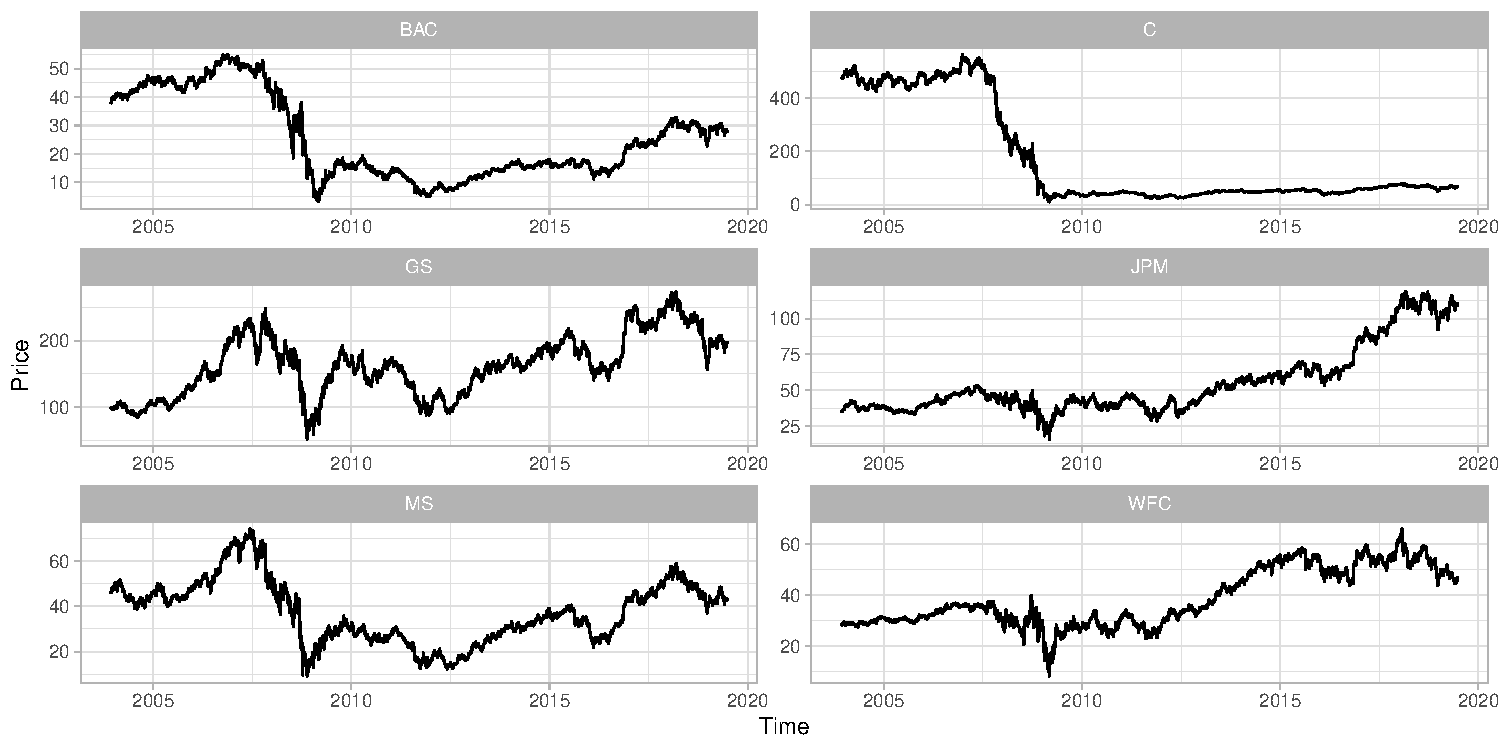
\includegraphics[width=\textwidth]{C:/rproject/EFRP/plot/unnamed-chunk-5-1.pdf}
  \label{fig1}
  \caption{Time-series used in this study.}
\end{figure}

\begin{figure}[ht]
  \centering
  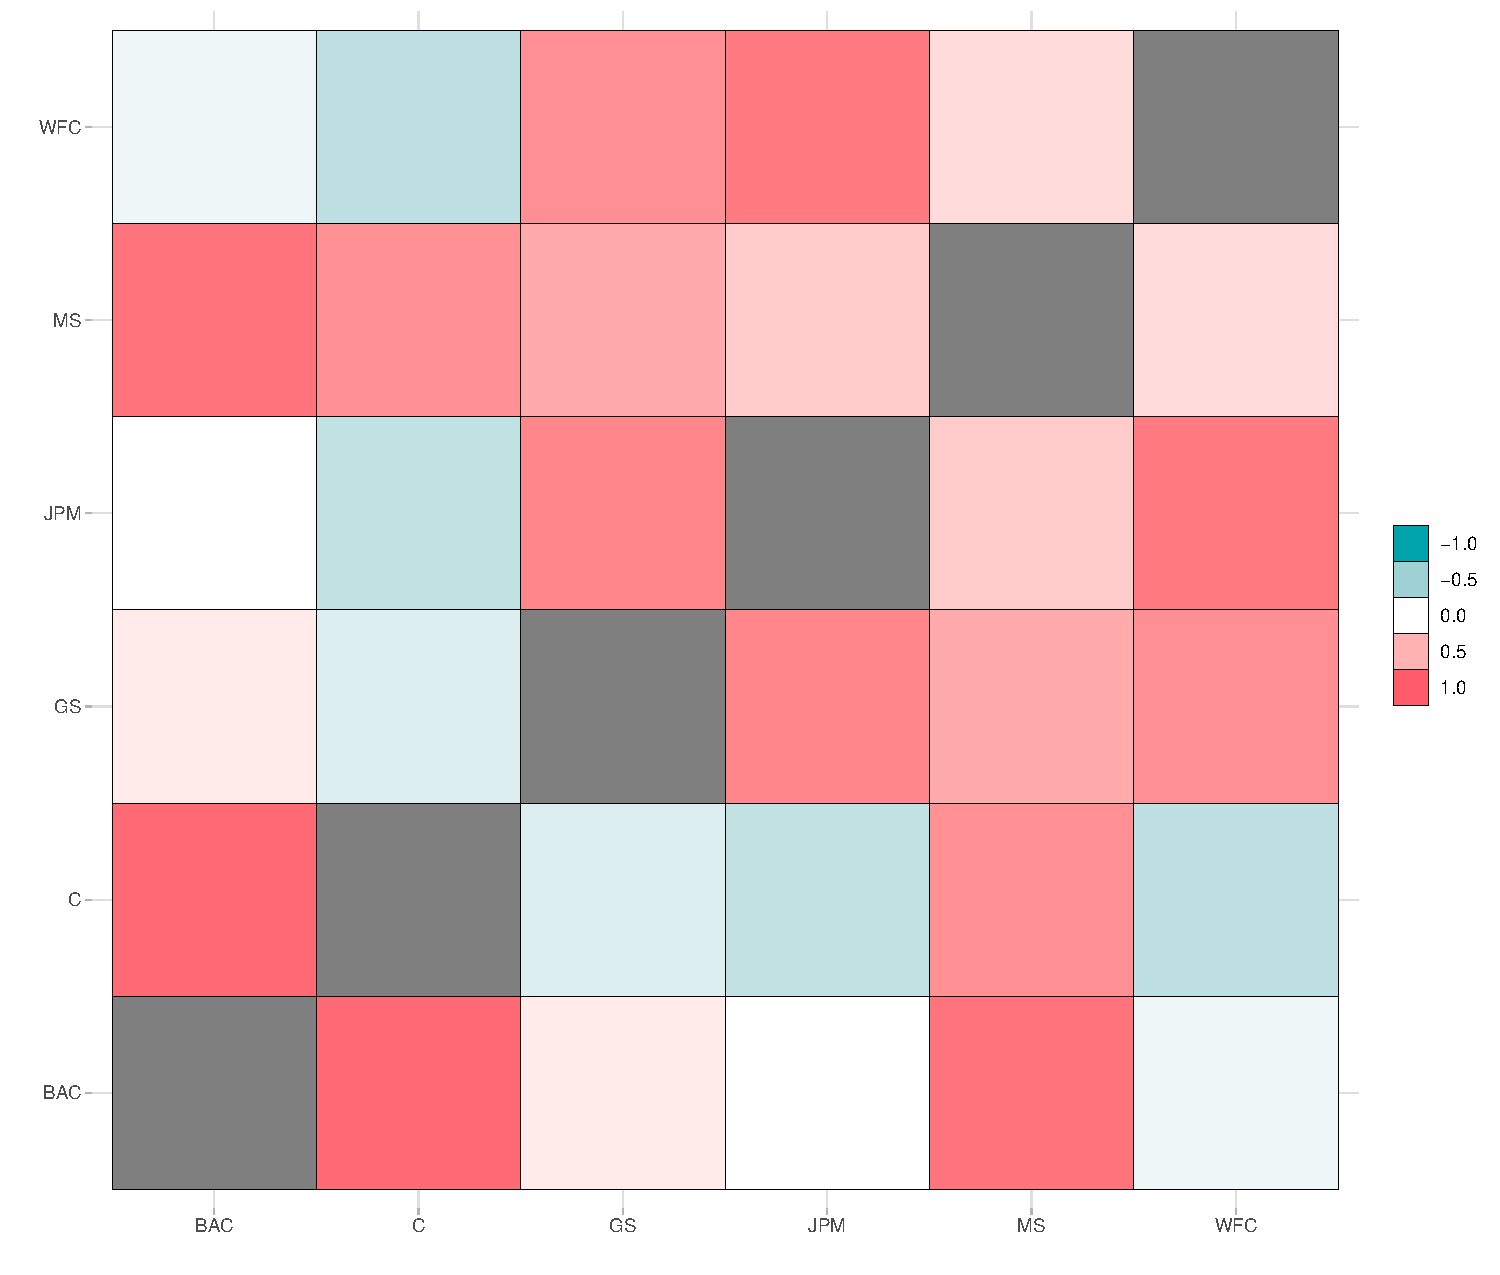
\includegraphics[width=\textwidth]{C:/rproject/EFRP/plot/unnamed-chunk-6-1.pdf}
  \label{fig2}
  \caption{Correlation-matrix.}
\end{figure}

\begin{figure}[ht]
  \centering
  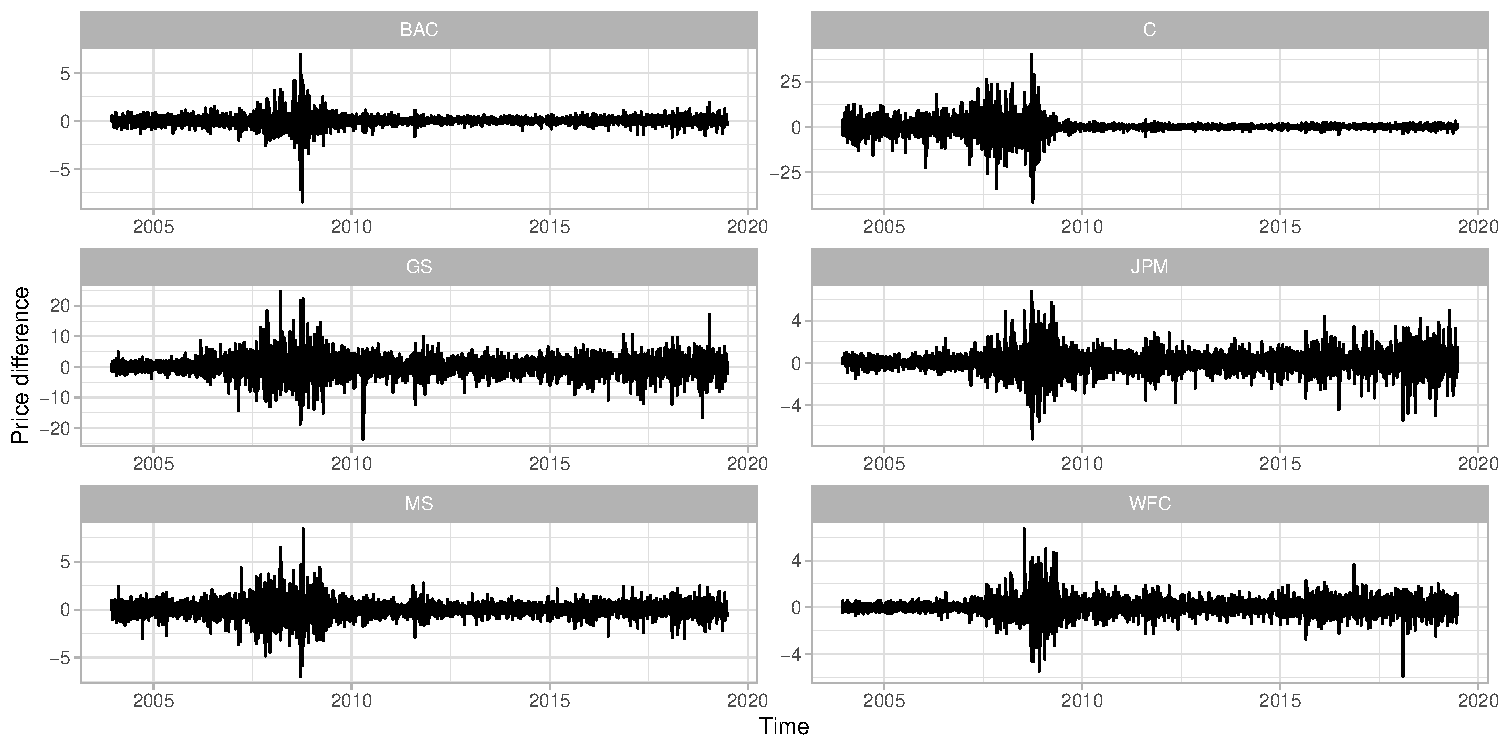
\includegraphics[width=\textwidth]{C:/rproject/EFRP/plot/unnamed-chunk-8-1.pdf}
  \label{fig3}
  \caption{First difference of the time-series.}
\end{figure}

\begin{figure}[ht]
  \centering
  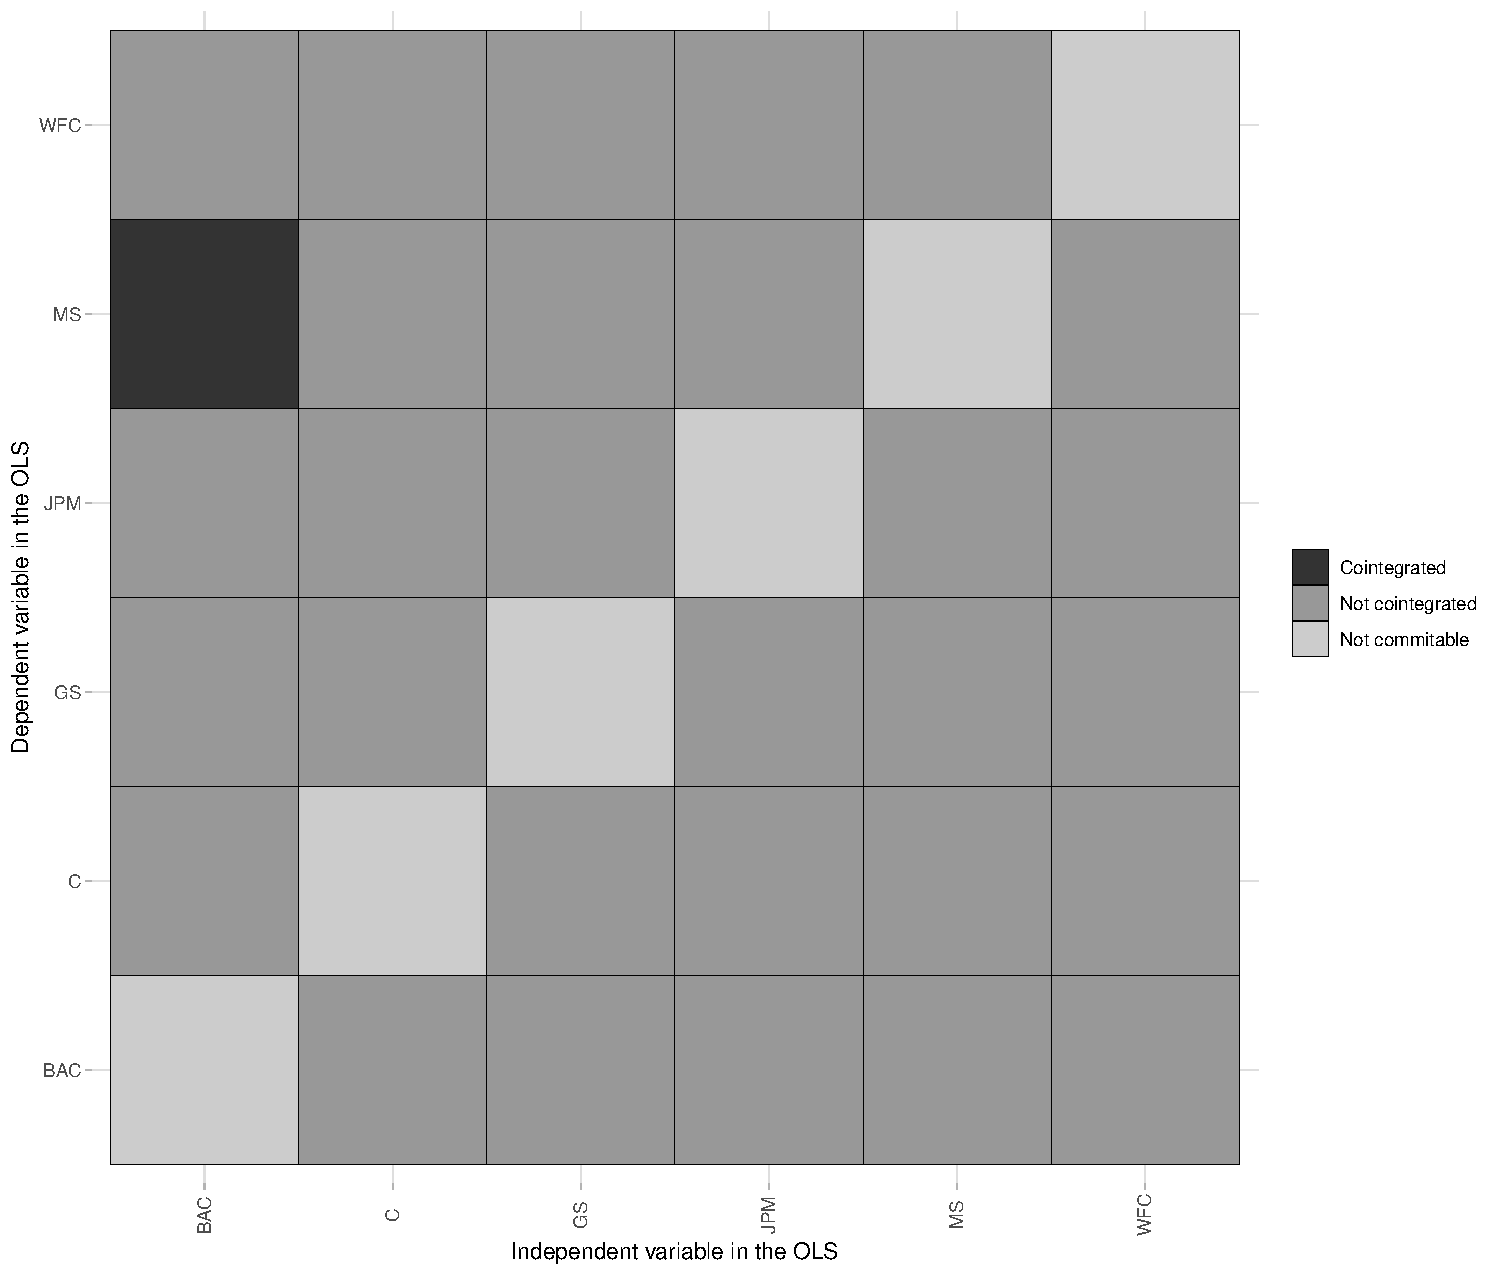
\includegraphics[width=\textwidth]{C:/rproject/EFRP/plot/unnamed-chunk-10-1.pdf}
  \label{fig4}
  \caption{Results of Engle-Granger method.}
  Calculations are based on ADF-test (level, $\alpha = 5\%$)
\end{figure}

\begin{figure}[ht]
  \centering
  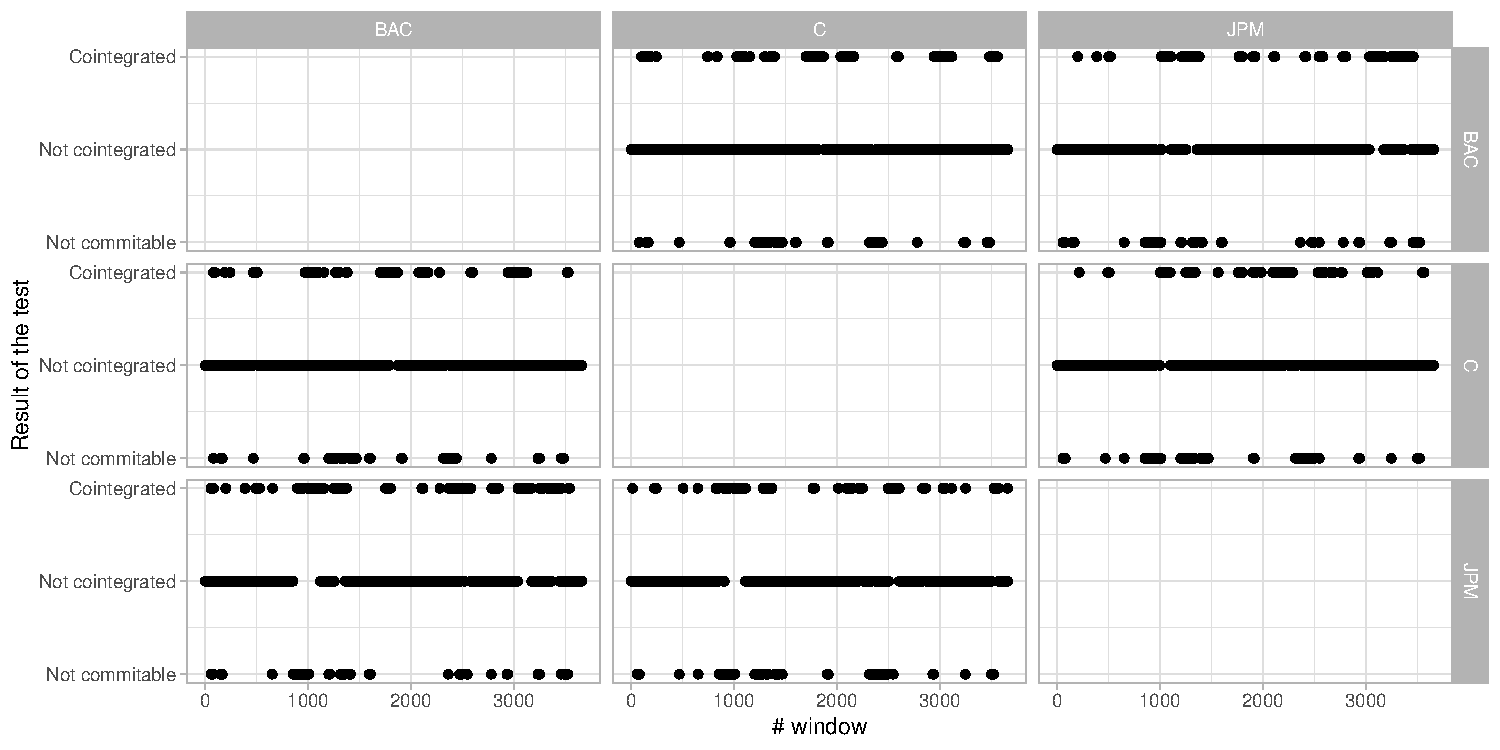
\includegraphics[width=\textwidth]{C:/rproject/EFRP/plot/unnamed-chunk-12-1.pdf}
  \label{fig5}
  \caption{Results of Engle-Granger method with rolling window.}
  $Size of windows = 250$. Calculations are based on ADF-test (level, $\alpha = 5\%$). Depedent variables (in the OLS) are placed horizontal, independents are vertical.
\end{figure}

\begin{figure}[ht]
  \centering
  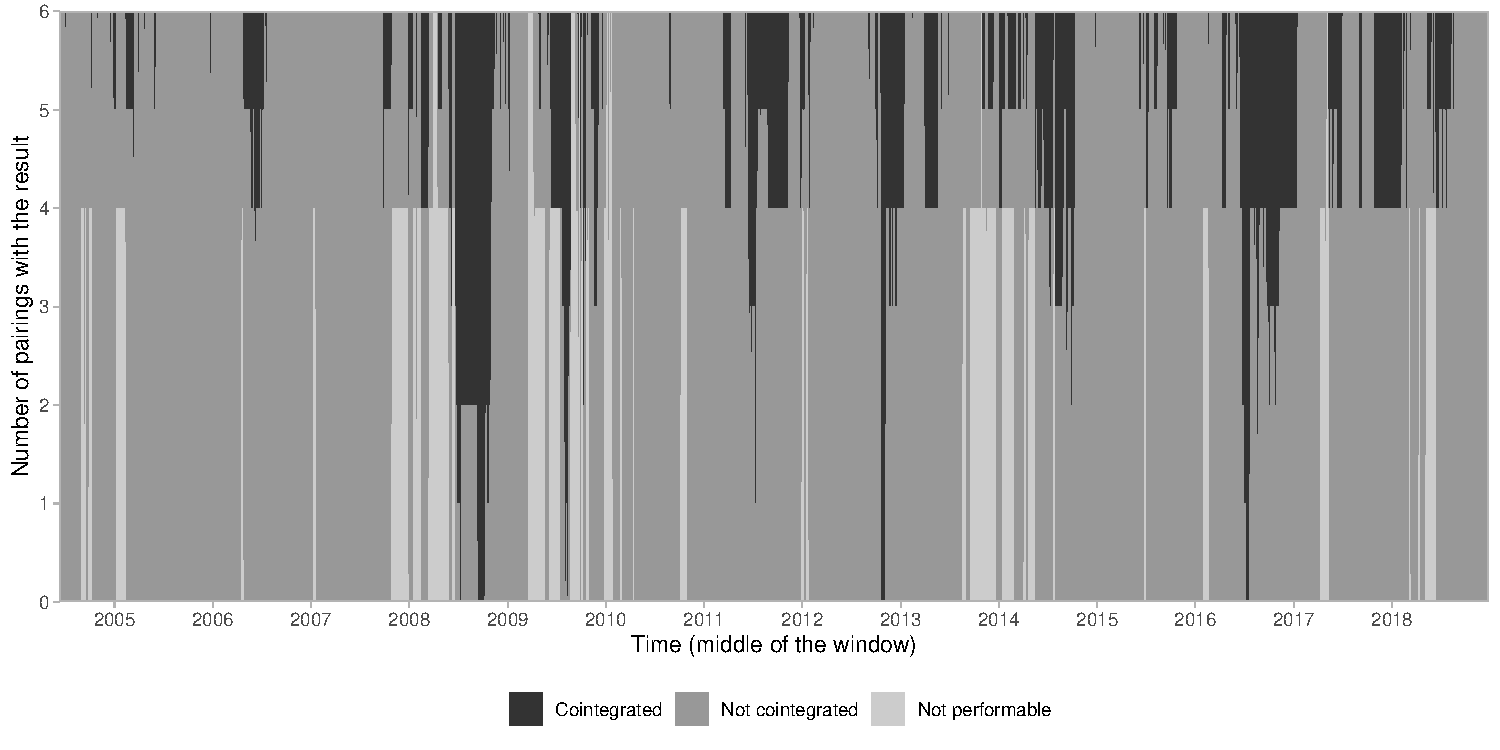
\includegraphics[width=\textwidth]{C:/rproject/EFRP/plot/unnamed-chunk-14-1.pdf}
  \label{fig6}
  \caption{Summary results of Engle-Granger method with rolling window.}
  Calculations are based on ADF-test (level, $\alpha = 5\%$). Number of total pairs is 6.
\end{figure}

\begin{figure}[ht]
  \centering
  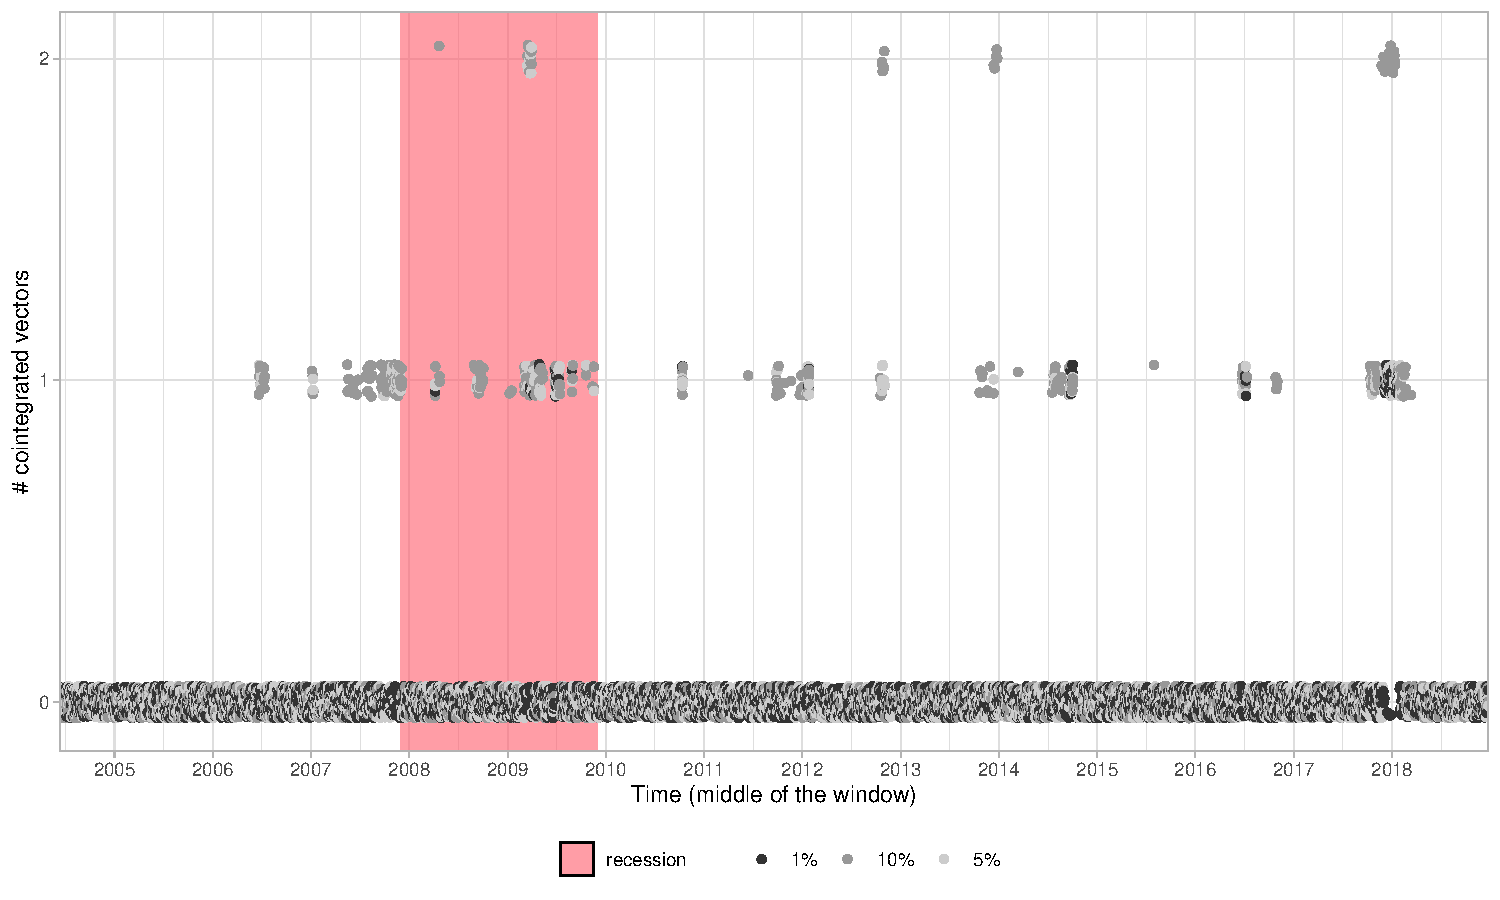
\includegraphics[width=\textwidth]{C:/rproject/EFRP/plot/unnamed-chunk-15-1.pdf}
  \label{fig7}
  \caption{Results of Johansen-test with rolling window across time.}
  $Size of windows = 250$. Points are jittered around their true y value for better visualisation (the number of cointegrated vectors is interger). Date of recession is from \href{https://www.nber.org/cycles.html}{the National Bureau of Economic Research}.
\end{figure}

\begin{figure}[ht]
  \centering
  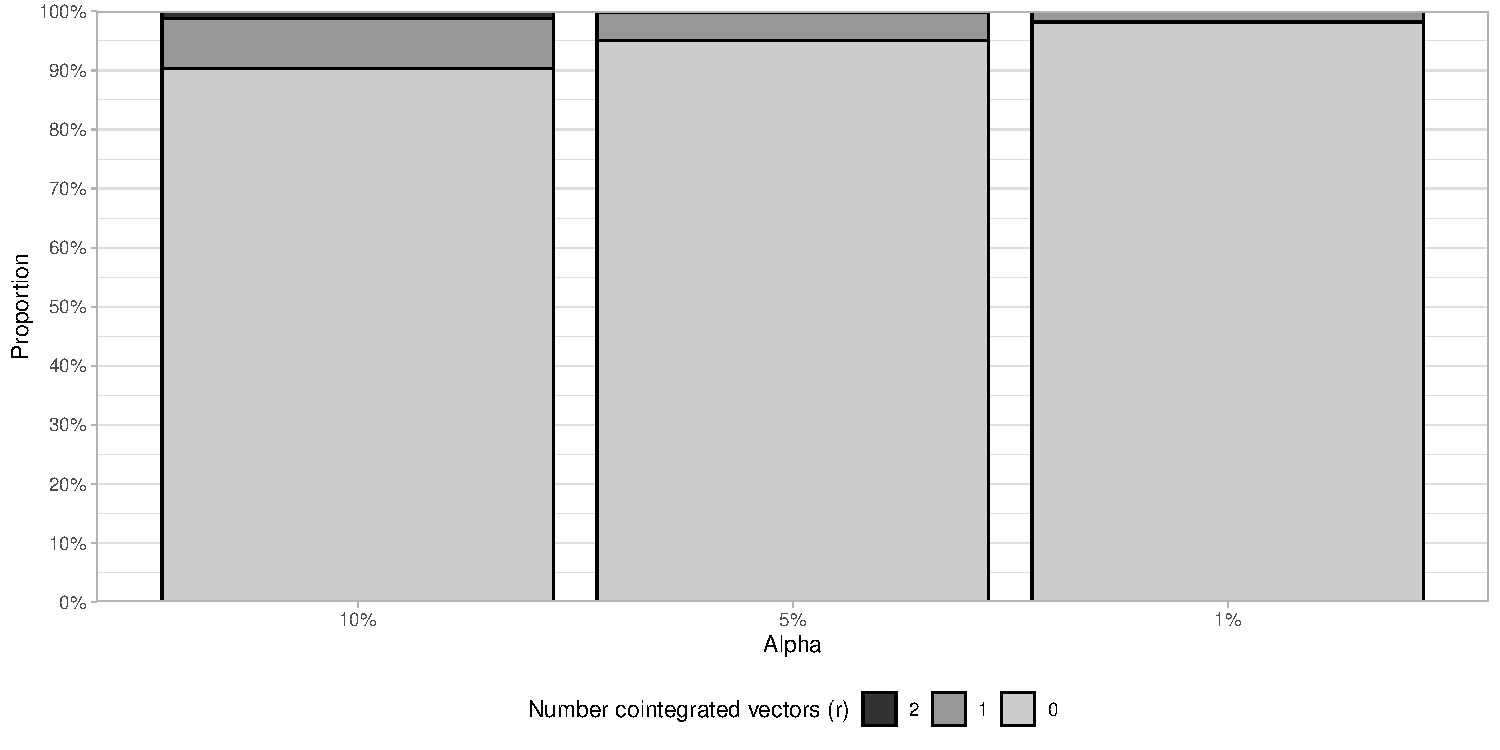
\includegraphics[width=\textwidth]{C:/rproject/EFRP/plot/unnamed-chunk-16-1.pdf}
  \label{fig8}
  \caption{Distribution of the Johansen-test results with rolling window.}
\end{figure}

Most %\cite{Huck.2014}
?

\begin{appendix}
  \listoffigures
  \listoftables
\end{appendix}

\bibliography{CointegrationBib}
\bibliographystyle{Apalike}

\end{document}